%
% Author kit for UCSC graduate classes in computer systems.
%
% Author guidelines and sample document in LaTeX 2e.
%

\documentclass[10pt,twocolumn]{article}

% Use the USENIX style file
\usepackage{usenix}

% Here are a bunch of useful packages
\usepackage{cite}
%\usepackage[]{biblatex}
\usepackage{xspace,verbatim}
\usepackage{subfig}
\usepackage{graphicx}
\usepackage{epstopdf}
\usepackage{float}
\usepackage{listings}
\usepackage[hyphens]{url}
%\usepackage{hyperref}
%\hypersetup{breaklinks=true}
%\urlstyle{same}
%\usepackage{url}
%\usepackage{tabularx}
%\def\UrlBreaks{\do\/\do-}
%\usepackage{breakurl}
%\usepackage[breaklinks]{hyperref}

% subfig default captions are too small.  This fixes it.
\captionsetup[subfloat]{font=normalsize}

% Redefine the percentage of the page that can be used for floats (figures,
% tables, etc.)
\renewcommand\floatpagefraction{.9}
\renewcommand\dblfloatpagefraction{.9}
\renewcommand\topfraction{.9}
\renewcommand\dbltopfraction{.9}
\renewcommand\bottomfraction{.9}
\renewcommand\textfraction{.1}
\setcounter{totalnumber}{10}
\setcounter{topnumber}{10}
\setcounter{dbltopnumber}{10}
\setcounter{bottomnumber}{10}

% Don't allow widows or clubs - single lines at the start/end of a column
\widowpenalty=10000
\clubpenalty=10000

\newcommand{\latex}{\LaTeX\xspace}
\newcommand{\unix}{\textsc{Unix}\xspace}

\pagestyle{plain}

%------------------------------------------------------------------------- 
\begin{document}

\title{Using SIMD Instructions to Accelerate Log-Structured Merge Operations}

\author{
{\rm James Byron} \\
\textit{jbyron@ucsc.edu}
}

\maketitle

\begin{abstract}
LSM trees are a widely used data structure in high-performance database systems.  As the size of LSM-tree-based databases grows, the operation of merging multiple arrays into a single array becomes increasingly demanding on computer systems, potentially slowing down database performance during the merge process.  CPUs have, in recent years, become more powerful with their ability to process multiple pieces of data in a single instruction.  SIMD instructions may be used to speed up many database tasks, including comparison and sort tasks.

In this paper, we introduce an algorithm that uses AVX2 instructions to perform the merging operation in an LSM tree.  We describe our algorithm's operation, the instructions it uses, and present its performance compared with a standard sorting algorithm from the C standard library.  Our results show that our current design does not beat the performance of the C library's qsort.  We describe further performance improvements that may enhance the performance of our merge algorithm.
\end{abstract}


\section{Introduction}
A recent report from the research firm IDC claimed that the amount of data globally will increase by 30\% annually through 2025~\cite{p3}.  As information systems become increasingly ubiquitous, the amount of information that databases must store is also increasing.  Large database systems that store large amount of information must also serve an increasing number of data queries.  While the need for data storage and access increase with the proliferation of information systems, the performance and capacity of individual computers may not keep pace with demand.

The need for increasing performance and capacity in databases drives a movement toward distributed databases.  Databases like BigTable and RAMCloud can run on hundreds or thousands of compute nodes to serve many thousands of simultaneous queries and puts to the database.  Increasing the number of compute nodes in the database can also increase its total performance; however, increasing the scale of distributed database systems also increases their capital and operational costs.

An alternative strategy to increasing the scale of database systems is to improve their efficiency.  Multicore processors, which enable multithreading in databases, can significantly increase the performance of a single computer, and modern databases routinely support multithreading to maximize the throughput of a single compute systems.  Multithreading is now common in database systems, and the performance of database systems depends largely on the efficiency of the database's design.

The log structured merge tree increases the performance of database systems by writing data to persistent storage in sequential blocks.  Hard disks, SSDs, and DRAM feature optimal performance when data is written in sequential blocks.  The LSM tree data structure optimizes a database by writing data to persistent storage in logarithmically increasing chunks of sorted vectors.  The sequential write operation minimizes the expensive seek time of hard disks or the write amplification in SSDs.  DRAM also reaches its fastest performance when reading and writing large chunks of contiguous data since processors retrieve entire cache lines with each random read.  The LSM tree trades small writes and seek operations in storage for the cost of sorting the vectors of keys before they are written to persistent storage.

LSM trees must sort the keys before they are written do disk or persistent memory in order to find a key without having to first search through the entire database.  Sorting the keys also allows LSM trees to update the values associated with keys without modifying the data already written to disk.  Sorting operations can be expensive, especially as the size of the data structures grows within the database.

Single instruction, multiple data (SIMD), which performs multiple operations on a block of data in a single instruction, may help to accelerate the process of merging multiple arrays of keys during an LSM tree merge operation.  SIMD instructions have become increasingly capable in recent processor designs as their number and variety have increased.  They operate on fixed-size vectors of values ranging from 32 bits to 512 bits in length.  In this paper we propose algorithms for merging pre-sorted arrays of keys into a single sorted array.  We measure the performance of our algorithms and compare them with a scaler design that does not use SIMD instructions.

The following sections include a summary of related work, an overview of our approach, a description of our implementation, experimental results, and a conclusion and future work.

\section{Related Work}
SIMD instructions are a promising research direction for database operations because they support bulk operations on data without requiring multithreading or multiple instructions.  SIMD instructions have also been applied to sorting algorithms that operate on an array of data.  Vector data operations require careful preparation of data and algorithm design in order to accelerate an application, and previous research using SIMD instructions have attempted to optimize a specific aspect of either database operations or sorting algorithms.  We discuss previous research related to SIMD instructions in databases and sorting in this section.

\subsection{SIMD in Databases}
SIMD instructions process multiple data values with a single instruction in one or a handful of cycles.  SIMD instructions were first popularized to accelerate multimedia applications, but later additions expanded the support for larger vectors and more operations.  Today, vector instructions can operate on 256 and 512-bit vectors to do operations like scaling, selection, and bit manipulation.  While vector operations are fast, the main challenge of using vector instructions is to efficiently import data into the vectors and to find instructions that can manipulate the data as needed.

Many data operations are difficult or impossible to support on today's hardware implementations.  Previous research has proposed adding new instructions or using existing instructions in novel ways to accelerate specific database operations.   Reinsel, Gantz, and Rydning~\cite{p1} introduce a variety of techniques for supporting database GroupBy operations with vector instructions.  They suggest adding new vector instructions to the x86 ISA that will allow manipulation of numerical data for database operations more easily and with more flexibility.  The authors use a simulator to predict the performance of database operations using their proposed instructions.  The proposed vector instructions provide a performance speedup of between 2.7x and 7.6x, depending on how the instructions are used.  

\subsection{Sorting Using SIMD Instructions}
Previous research has addressed the possibility of utilizing SIMD instructions to accelerate sorting algorithms~\cite{p13}.  Traditional scaler designs compare two values at a time.  SIMD approaches can improve performance between and 20x~\cite{p11} and 270x~\cite{p10}.  New instruction set extensions that support more vector operations on larger bit arrays will further improve performance.   The AVX512 instruction set, which today is available on a limited number of Intel CPUs, improves the power of sorting algorithms.  Inoue and Taura~\cite{p12} analyzed current sorting algorithms and proposed vector instructions that could further accelerate the sorting of integers and key-value pairs.  

SIMD-enhanced sorting algorithms rely on rapid translation of program data into vector data structures and back.  In some programs, the translation occurs as a cast from one an integer or other data type to the vector data type.  Casting program data into vector data types applies when the data to be sorted is stored in a contiguous block of memory.  Some sorting algorithms must sort arbitrary data structures that are not present in contiguous blocks to memory, and the data must first be copied into SIMD vectors before it can be processed.  This slows down the sorting algorithm, possibly eliminating any advantage from using the vector instructions.

\subsection{Log-Structured Merge Tree}
The Log-Structured Merge Tree was initially proposed as a technique to optimize large scale data center storage and balance the high cost and fast performance of RAM with relatively low-cost and slow disk-based persistent storage~\cite{p4}.  The LSM approach has been applied in many database designs, including BigTable~\cite{p5}, RAMCloud~\cite{p6}, Cassandra~\cite{p8}, and RocksDB~\cite{p7}.  Log structures have also been used to accelerate writes to data in DRAM, since even DRAM provides much faster throughput when reading and writing to large blocks at a time~\cite{p9}.

\section{Approach}
In this section we define our motivation and the problem that we attempt to solve, the alternative solution that is currently in use, an overview of SIMD instructions, and a description of how we apply them to LSM tree merge operations.  In this paper, we use the terms \textit{log}, \textit{array} and \textit{data component} interchangeably to refer to the data structures in the LSM tree.

\subsection{Problem Background}
LSM trees are an efficient data structure that is optimized for databases that require the ability to write data quickly.  Write operations add to data structures called arrays that are sorted by key.  Initially, the LSM tree consists of small in-memory arrays to which keys are appended as the user writes data to the database.  Data in the arrays is written to disk in sorted ascending order and stored in the small sequential arrays that fill up as data is added to them.  When the initial arrays are full of data, the database is briefly paused to merge the small initial arrays into a single large array that combines all their keys into one sorted component.  When more data is appended to the database, new array components are created, filled, and recursively merged into other arrays that grow in length as the size of the database grows.

We reference the number of levels in an LSM tree as its depth.  The arrays at each level in the tree must be large enough to store the data in all of the arrays of the preceding level.  Thus, we say that the length of the arrays grows exponentially as the depth of the tree increases.  We describe the length of array components formally using the formulas:

$$Length(i+1) = length(i) * ArraysPerLevel$$
$$Length(i+2) = length(i+1) * ArraysPerLevel$$
$$length(n) = length(0) * ArraysPerLevel^(depth-1)$$

The configurable parameters for an LSM tree are the length of the arrays in the first level of the tree, level 0, and the length of the arrays at level 0.  The number of arrays in each level of the tree determines the rate of exponential growth for the LSM tree data components.  One possible implementation-and the approach that we have used in our implementation and testing-is to use ten arrays for each level in the tree.  We also test the performance of our algorithm using two, four, six, and egiht data components at each level.  The length of the arrays in the first level of the tree impacts the computational cost of adding data to the LSM tree.

Our design requires that the array data components at each level of the tree remain sorted as data is added to them.  We call this property invariant 1.

\textit{Invariant 1: The keys in each array of the LSM tree are sorted in ascending order.}

The purpose for this invariant is to enable key lookups without requiring a scan of the entire LSM tree data structure.  With the keys in sorted order, we search for a key by scanning each log data structure from right to left, or from the greatest to the least key.  We abort a search for a key within a log when the keys in the log are less than the key that we are searching for.  In the worst case, when searching for a key that is not in the database, this approach still requires a complete scan of the LSM tree; however, when scanning for keys that were recently added to the database, this simple lookup approach scans a minimal number of keys to deterministically retrieve the desired key.  We discuss potential improvements to this lookup operation in the section devoted to future work.

While invariant 1 supports fast lookups of stored keys, the process of merging levels of the LSM tree must preserve this invariant.  The baseline approach to merging multiple logs involves simply concatenating the logs of a level of the tree and sorting the resulting log.  Sorting algorithms compare pairs of numbers to sort lists of values.  Fast sorting algorithms like quick sort and merge sort require $O(n\textit{log}(n))$ comparison operations to create a sorted list.  We present an alternative approach that compares multiple values simultaneously using SIMD instructions.

\subsection{SIMD Instructions for Sorting}
Merging the logs of an LSM tree requires preserving the invariant that each log is sorted by key from least to greatest.  Since the logs that are an input to the merge algorithm are already sorted from least to greatest, we know that the greatest key in a set of logs is at the right end of one of the logs.

We use SIMD instructions to compare the keys of the logs to find the single maximum key.  To merge multiple logs, we repeatedly select and merge the maximum value from all the logs until all of the values in the input logs have been selected and inserted into a new output log.

Intel AVX instructions~\cite{p2} include operations that compare two vectors of integer values.  Each vector is 256 bits in length, which is large enough for two 128-bit quadruple length integers, four 64-bit double length integers, eight 32-bit integers, sixteen sixteen-bit short integers, or 32 eight-bit half short integers.  We use 32-bit integer values throughout our experiments, allowing each vector to store eight integer values from our logs.   For the purposes of this discussion, a log refers to the sorted keys, which are represented as integers, and a vector refers to a group of eight integers that have been extracted from a sorted log.  The AVX instruction set includes instructions that allow us to insert eight integer values into a vector with one instruction.

SIMD comparison instructions return a vector of the maximum or minimum values from two input vectors of numbers.  The values in the input vectors are compared in corresponding pairs so that each integer in the resulting vector is the maximum or minimum of the integers in the same position of the input vectors.  The comparison is non-destructive of the original bit vectors, so after finding the maximum values of a pair of vectors with one instruction, we can also find the minimum values with one more instruction.  Thus, we can find the minimum and maximum integer values of two vectors using two instructions:

$$newA = max(A, B)$$
$$newB = min(A, B)$$

Here, A and B are the input vectors, each containing eight integers in ascending order.  NewA and NewB are the new vectors containing the maximum and minimum values corresponding to each index in the vectors.  Therefore, after executing the $max$ instruction, the NewA vector will store at each index \textit{i} the maximum value from vectors A and B at index \textit{i}.  The $max$ and $min$ instructions operate on vectors of integers by sorting their values within each column of integers.  The instructions do not rearrange the integers within each vector.  For this reason, the $max$ and $min$ instructions do not violate invariant 1 as defined earlier.

To find the largest key within any pair of logs, we sort the vectors containing the keys using the SIMD instructions for comparison.  Similarly, we find the maximum key of a set of ten logs during a merge operation by comparing each pair of logs twice to get the minimum and maximum vectors until the maximum key is in the top-most integer vector.  For three or more vectors, we say that:

$$newA = max(A, max(B, ... Z))$$

After each call to $max$ to get NewA, we also call $min$ with the same input vectors to get NewB in order to preserve the minimum keys for the next iteration of the sorting algorithm.  With two vectors, we must perform two comparison operations to move the larger keys to the top vector and the smaller keys to the bottom vector.  With three vectors, we must perform four comparison operations.  With four vectors, we must perform six comparison operations, and with ten vectors, we must perform 18 comparison operations.

Rather than finding the maximum integer key from a set of vectors, we can instead find the minimum integer of a set of vectors using the SIMD comparison instruction for minimum value:

$$newZ = min(Z, min(Y, ... A))$$

We observe that to move the maximum or minimum integers of a set of vectors to the top vector or bottom vector respectively, we must compare each pair of vectors twice to get the minimum and maximum keys starting at either the bottom or top vector.  Finding the maximum integers must sort starting at the bottom vector, and finding the minimum integers must sort starting at the top vector.

As we describe in the next section, we chose to select the maximum integer of a set of vectors rather than the minimum value of a set of vectors.  We discuss possible optimizations to our approach in the section for future work.

\subsection{Selecting the Maximum Key}
We can find the maximum integer within ten vectors using 18 SIMD instructions.  We call this one sorting pass.  When starting with the bottom vector and sorting each pair of vectors till the top vector, the maximum integer within each column of integers in the vectors will move to the top vector.  Thus, all of the integers in the top vector are greater than the integers in the corresponding columns of the vectors below them.  By invariant 1, they are also greater than the integers to their left.

After completing one sorting pass from the bottom vector to the top, we have selected only the maximum values within each column of integers.  To select the minimum values in each column of integers within the vectors, we must sort starting at the top and proceed to the bottom.  Thus, sorting for the minimum integer will also require 18 instructions.  Since the two sorting techniques must work in opposite directions, they do not do the same work, and we cannot extract minimum values from the bottom vector after sorting bottom-to-top for the maximum integer key.  In our design, we select only one (maximum) integer at a time using the bottom-to-top sort to find the maximum integers.

We recall that, by invariant 1, all values in each log are sorted in ascending order from left to right .  After a group of vectors is sorted so that the maximum integer keys are in the top row, we say that, by invariant 1, the maximum key in all vectors is at the right-most column in the top vector.  We select the integer in the right column of the top vector and add it to the end of our merge output.

\subsection{Shifting keys}
After selecting an integer key from the vectors and merging it with the output log, we next shift the integers in the top-most vector by 32 bits to the right.  This action moves the second integer in the top vector to the first position in the top vector.  The integer in the left-most column becomes 0.  We replace the 0 value of the left-most integer with the values from the right-most vector of the next group of vectors to the left.

Recall that each vector stores exactly eight 32-bit integer keys.  When the logs are more than eight integers long, we maintain a separate group of vectors for each group of eight keys within the input logs that we are merging.  Therefore a log with eight integers will require one vector, and a log with 80 integers will require ten vectors.  We arrange the vectors in the same order as their corresponding keys in the group of 10 input logs to the sorting algorithm.  We also manipulate each additional group of ten vectors in the same way that we manipulate a single group of vectors.  After loading the log keys into the vectors, we sort each group of vectors, select the integer in the right-most column of the top vector, and shift all the integers in the top vectors by 32 bits to the right after copying the greatest value from the right-most vector into our output log.  We repeat this process until we have merged all integer keys into the output log.



\section{Implementation}
We have implemented our sorting algorithm in C using the AVK and AVX2 instruction set extensions.  We therefore assume that any computer used to execute our code will have the AVX and AVX2 instruction sets, which are features that have been included in Intel CPUs since the Haswell generation of Core processors.  Also, the C programming language includes many \textit{intrinsic} functions that translate correctly-formatted C code into the corresponding assembly instruction that can run on a CPU with AVX and AVX2 instruction sets.  We describe the instructions used in our implementation below.  The code for this project is available on GitHub at \url{https://github.com/JamesByron/CMPS278-Project}.

\subsection{Data Types}
The log data structures are represented as integer arrays.  The SIMD instructions support a variety of other numerical formats for both integer and floating point values.  The vector instructions in our implementation utilize the \textit{m256i } data type, which is a 256-bit vector containing 32-bit integers.

\subsection{Loading}
The loading operation copies all of the integer keys from the logs into 256-bit vectors containing eight 32-bit integers.  We used the intrinsic instruction \textit{mm256setrepi32}, which we call with eight integer arguments taken from the logs that we are merging.  The setr instruction copies the integers into memory in the reverse order from the arguments.  The x86 instruction set is big-endian, and in order to simplify the translation between log indices and vector indices, we use the reverse ordering instruction and index them in the same way.  The setr instruction returns a \textit{m256i } vector.  We store the vectors for the logs in an array of \textit{m256i}.

\subsection{Comparison}
The AVX2 instructions for $max$ and $min$ are \textit{mm256maxepi32} and \textit{mm256minepi32}, respectively.  Each instruction takes as arguments two \textit{m256i} integer vectors and returns a new vector of either the maximum or the minimum values.  We replace the \textit{m256i} vectors in the array of vectors with the new minimum and maximum vectors returned by the maximum and minimum intrinsic functions.

\subsection{Extracting and Inserting}
We use the AVX extraction intrinsic function to retrieve a value from a \textit{m256i} vector before shifting its integers.  The intrinsic function for extraction is \textit{mm256extractepi32}, which takes as arguments an \textit{m256i} vector and an index to extract from the vector and return as an integer.

We use the AVX insert intrinsic function to insert integers into the bit vectors during the shifting operation.  The insert function is \textit{mm256insertepi32}, and it takes a \textit{m256i} vector, the integer value to insert into the vector, and an index of the position to insert the value.  The insert function returns a new vector with the integer inserted at the location corresponding to the index.

\subsection{Shifting}
There is no single instruction in the Intel architecture that can shift an entire 256-bit vector by 32 bits.  Instead, we have selected an instruction that shifts 128 bit lanes by a specified number of bytes.  We use the AVX2 instruction \textit{mm256sllisi256} to shift both halves of the vector left by 32 bits.  When shifting left, we again recall that Intel's big-endian ISA will result in the integer values moving to the right to facilitate easy translation between the indices of keys in our logs and the vectors.  To complete the shifting operation, we extract the integer at position 3 within the vector and insert it into position 4 after the shifting has completed.  The extract and insert operations are necessary to save the integer at the end of the first 128-bit lane boundary of the vector that otherwise would be lost if not copied into the vector after shifting.  The final vector has an integer of 0 in its first integer position, the right-most integer removed, and all other integers shifted to the right.

\subsection{Testing Framework}
We evaluate our SIMD merging algorithm by generating sorted lists of integers and passing them to the SIMD merge algorithm.  We evaluate the time to complete the merge operation as the length of the input logs grows.  With the goal of further testing and development, we have implemented a communication socket that will communicate with another program through IPC or over the network port to store and retrieve values from clients.  We have not used the IPC socket for the purposes of our experimental testing in this paper, but we leave that to future work.

\section{Experimental Results}
Our goal is to compare our merge algorithm with a more conventional merge-and-sort approach, we measure the time to merge a set of array data components as their size increases.  We compare the merging operation using SIMD with a sorting algorithm qsort from the C standard library.

\subsection{Time To Merge}
\begin{figure}
\label{f2}
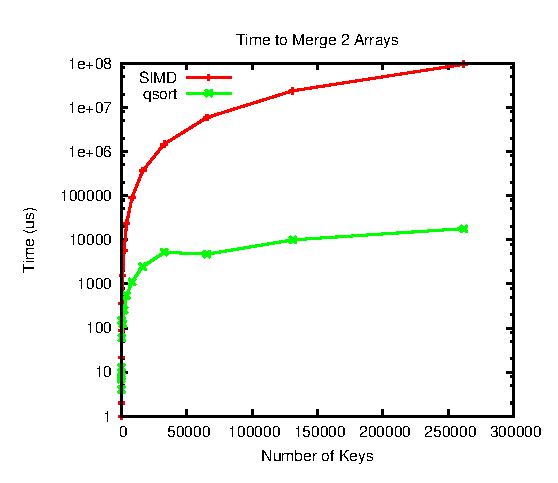
\includegraphics[width=\linewidth]{2.eps}
\caption{We measure the time in microseconds to merge two arrays of data using SIMD instructions and the qsort algorithm from the C library.}
\end{figure}

Throughout our experiments, we vary the number of arrays that the algorithms must merge, and we measure the amount of time taken for the sorting function to complete.  The time in each groph shows how long it took for the sorting algorithm to complete during a single merge operation.  The time values are not cuumulative.

\begin{figure}
\label{f4}
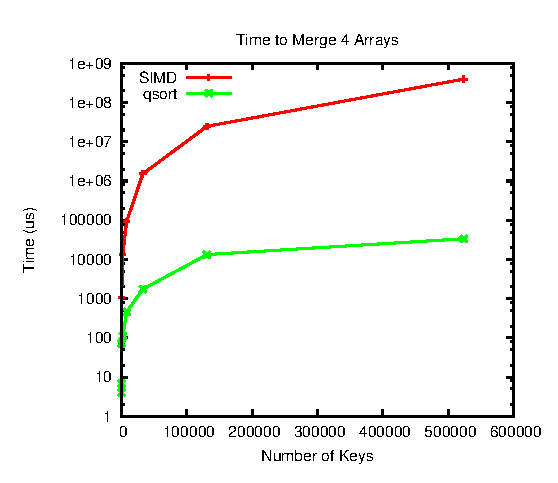
\includegraphics[width=\linewidth]{4.eps}
\caption{We measure the time in microseconds to merge four arrays.  The time increases as the total number of keys increases.}
\end{figure}

Figures 1 through 5 suggest that the SIMD merge algorithm requires much more time to merge large arrays than qsort from the C standard library.  We discuss our observations further in the next section.

\begin{figure}
\label{f6}
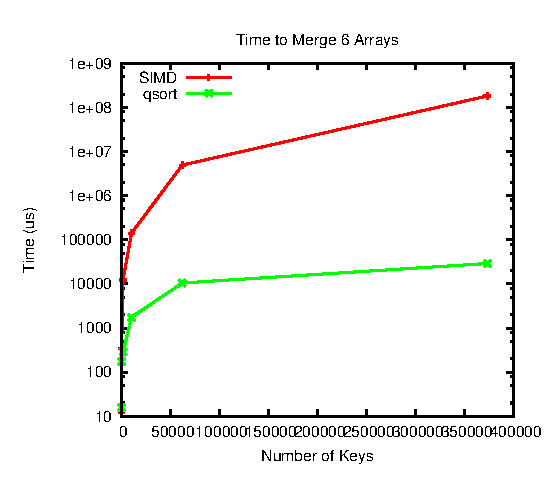
\includegraphics[width=\linewidth]{6.eps}
\caption{We measure the time in microseconds to merge six arrays.}
\end{figure}

\begin{figure}
\label{f8}
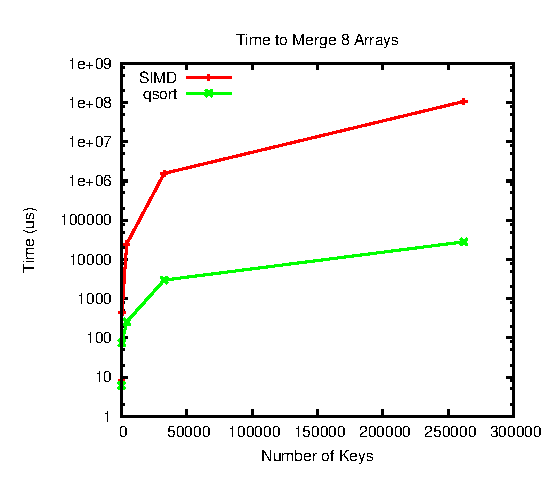
\includegraphics[width=\linewidth]{8.eps}
\caption{Changing the number of arrays to merge does not affect the relative performance of SIMD merge and qsort.}
\end{figure}



\begin{figure}
\label{f10}
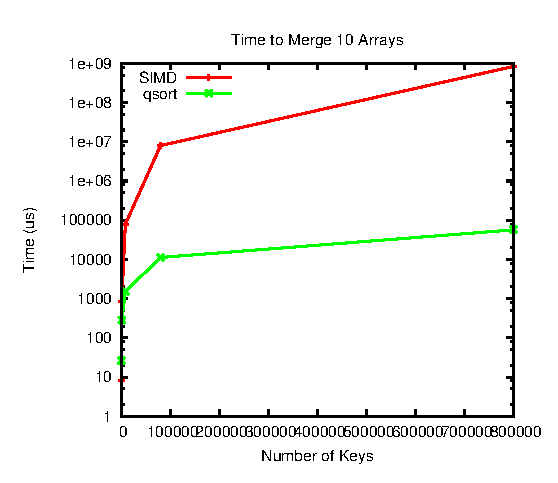
\includegraphics[width=\linewidth]{10.eps}
\caption{LSM tree implementations may merge ton arrays at a time.  The time to merge 10 arrays proves that our SIMD algorithm does not outperform a more conventional sorting algorithm.}
\end{figure}

\section{Discussion}
We have seen that merging arrays of integer keys using our SIMD algorithm does not outperform the baseline sorting algorithm from the C standard library.  The qsort algorithm is not optimized for the special case of merging multiple sorted arrays, yet it outperformed the design that we created with SIMD instructions.  We can find two reasons for this based on the observed performance of our merging algorithm.

\subsection{Time Complexity}
We have used SIMD instructions to perform comparison operations to sort groups of vectors.  While our approach successfully merges the input arrays, our algorithm has the added burden to resort many vectors that may not need to be compared and sorted at each step.  In this way, we are wasting computation time in order to ensure that our sorting algorithm correctly compares and every key.  When the number of keys increases, the SIMD merge algorithm requires an exponentially increasing amount of time to complete.  The exponential increase in time suggests that our merge algorithm performs $O(n^2)$ comparison instructions, while conventional scaler sorting algorithms typically require $O(n \textit{log}(n))$ comparison instructions.  The $n^2$ complexity or our merge sort algorithm comes from the fact that we resort each group of vectors after extracting each key.  Our SIMD algorithm is thus within a constant factor of exponential, and the power of SIMD operations helps to limit the number of distinct comparison operations.

When the total number of keys and resulting length of each array is small, the performance of SIMD sort is close to that of qsort.  We attribute this to the inherent imprecision of measuring time on a computer rather than any meaningful advantage of the SIMD merge algorithm.

\section{Future Work}
We have identified several avenues for future work to explore possible strategies to optimize the SIMD merge operation.

\subsection{AVX512}
Intel has published the specification for the next iteration of AVX instructions to process 512 bit vectors.  The new ISA, called AVX512, is currently available in the Intel Knight's Bridge CPU, and it will likely appear in future iterations of Core and Xeon processors.  AVX512 will process twice as much data with one instruction as AVX2 or its predecessors, and this will result in performance that is roughly double what is currently available with AVX2 for some instructions.  In particular, the intrinsic functions for load, compare, and shift will require half as many instructions as AVX2.  We therefore expect that AVX512 will provide some speedup over AVX2 with our design, and this implementation would possibly make SIMD merging more competitive with alternative sorting algorithms.

\subsection{Optimizing Key Lookup}
The worst case of a key lookup currently requires a complete scan of the entire database to verify that a key is not in the database.  Our current implementation uses the sorted ordering of logs to stop scanning the log when its keys are less than the key being sought.  This operation runs in worst-case time $O(n)$.  A more optimal searching algorithm will start searching for a key in the middle of each log.  If the value there is less than the key being sought, recursively search from the current index to the maximum index of the log.  If the value at the current index is greater than the value being sought, recursively search from the first value of the log up to the current index.   Since it leverages the sorted order of the log to search the half of the log remaining after each successive iteration of the search, this lookup strategy has a time complexity of $O(\textit{log}n * r)$, where \textit{n} is the length of the longest log in the database, and \textit{r} is the total number of logs in the database.  A further optimization would be to divide the entire database into two halves, one for odd keys and the other for even keys.  When searching for a key in such a database, the typical complexity would be $O((\textit{log}n * r)/2)$, assuming that the keys are evenly distributed between even and odd keys.  While not essential to the database's core functionality, they could significantly enhance its performance in some workloads.

When imagining these search algorithms, we recall that LSM trees are optimized for storage devices that feature high latency to random access data and high throughput for sequential access.  Our future work would sook to find the boundary of when it is more economical to conduct a linear search rather than a tree-based search.  The boundary would necessarily depend on the performance of the underlying storage system being used, since some storage devices like SSDs feature comparatively faster seek times than hard disks.

\subsection{Extracting Minimum Value}
In the SIMD merge algorithm that we have implemented, we extract one integer from the top vector in a column to add it to the merged output log.  We do not currently extract integers from the bottom row of the left-most column in the vectors, which is the position of the key with the lowest value when sorting top-to-bottom for the lowest key.  We may, however, be able to use this minimum value by waiting to extract minimum values until after completing $r-1$ sorts of each block of vectors, where \textit{r} is the number of logs that are being merged.  After $r-1$ bottom-to-top sorts, the minimum values in each block will also have reached the bottom of the groups of vectors.  We will also need to device a solution to the problem that the bit shifting introduces integers that will be sorted as the minimum value in the group of vectors.  By solving these challenges, we expect that our current SIMD merge algorithm would be approximately twice as fast as it is currently.

\section{Conclusion}
We have introduced an algorithm to merge the logs of an LSM tree using SIMD instructions.  Our algorithm relies on the latest widely-available instructions for 256-bit vectors. Our implementation demonstrated that AVX2 instructions can efficiently sort 16 values with two instructions or 80 values with 18 instructions; however, when applied to the application of merging multiple arrays of sorted data into one array of sorted data, our design required significantly more time than the qsort algorithm from the C standard library.  With the goal of improving on our design, we described ideas and techniques to explore other improvements that could enhance our algorithm's performance.






\section*{Acknowledgments}
I would like to acknewledge Shel Finkelstein for his guidance and sheparding throughout this project.

\bibliographystyle{abbrv}
\bibliography{refs}

\end{document}\grid
